\documentclass[article]{amsart}
\usepackage[margin=2cm]{geometry}
\usepackage{graphicx}
\usepackage{enumitem}
\setlist[description]{}
\usepackage{hyperref}
\usepackage{fancyhdr}
\usepackage[utf8]{inputenc}
\usepackage{listings}

\hypersetup{
  colorlinks=true,
  linkcolor=blue,
  urlcolor=cyan,
  linktoc=all
}


\pagestyle{fancy}
\fancyhf{}
\rhead{\thepage}

\begin{document}
\thispagestyle{empty}
\title{
	Simulaci\'on de eventos discretos \\
	n servidores en paralelo
}
\author{Chavely Gonz\'alez Acosta C412}
\date{\today}
\maketitle
\pagenumbering{gobble}

\newpage

\pagenumbering{arabic}

\tableofcontents

\pagestyle{fancy}
\newpage

\section{Introducci\'on}

\begin{enumerate}
\item \textbf{Breve descripción del proyecto} \\
El sistema a simular en el presente proyecto consiste en: m clientes, los cuales llegan a un sistema que tiene n servidores, con tiempo entre los arribos que distribuye M. Cuando un cliente llega, se une a la cola si ambos servidores est\'an ocupados. El caso de solo tener dos servidores se describe a continuaci\'on: Si el servidor 1 est\'a libre, el cliente entra en servicio con el servidor 1. Si el servidor 1 está ocupado pero el servidor 2 está libre, el cliente entra en servicio con el servidor 2. Cuando un cliente completa el servicio con un servidor (no importa cuál), ese cliente luego abandona el sistema. El cliente que ha estado en la cola durante más tiempo (si hay clientes en la cola) entra en servicio. La distribución de servicio en el servidor i es $ G_{i} $\\
\item \textbf{Objetivos y metas} \\
El objetivo fundamental de este proyecto es simular correctamente el sistema antes descrito y arribar a conclusiones como el tiempo promedio que pasa un cliente en la cola, el porciento de clientes que tienen que esperar para ser atendidos y el porciento de ocupaci\'on de cada servidor.\\
\item \textbf{Variables que describen el problema} \\
 Las variables de interés para este proyecto incluyen el tiempo entre los arribos de los clientes, la distribución de los servidores ocupados y la duración del servicio en cada servidor.\\
\end{enumerate}
\newpage
\section{Detalles de implementaci\'on}
La implementación de la simulación de eventos discretos se basa en los siguientes pasos:
\begin{enumerate}
\item \textbf{Modelado del sistema}\\
El sistema se compone de:
\begin{itemize}
\item Un conjunto de m clientes que arriban con una diferencia de tiempo que distribulle M y requieren alg\'un servicio\\
\item n servidores: $s_{1}, s_{2}, s_{3}, ..., s_{n-1}, s_{n}$, los cuales trabajan en paralelo y el tiempo que tardan en completar un servicio distribulle $G_{i}$\\
\item Una cola(FIFO) de clientes, inicialmente vac\'ia, para mantener a los clientes en espera mientras est\'an llenos todos los servidores hasta que se vac\'ie alg\'un servidor\\
\item En todo momento el servidor al cual se le asigna un servicio nuevo es, de los que no est\'en ocupados en ese momento, el de menor \'indice.\\
\end{itemize}

\item \textbf{Generaci\'on de eventos}\\
Para generar las variables aleatorias se utilizan los m\'etodos del m\'odulo de python $numpy.random$. Las distribuciones propuestas son las siguientes: poisson, geom\'etrica, uniforme, binomial, exponencial, normal, beta y ganma, con sus respectivos par\'ametros predefinidos por el propio programa. Al momento de relizar la simulaci\'on se decide cual(es) utilizar.\\
\begin{itemize}
\item Variables aleatorias: distribución de llegada de los clientes (M) y las distribuciones de servicio en los servidores ($G_{i}$)\\
\end{itemize}
\item \textbf{Procesamiento de eventos}\\
Para simular los eventos: llegada de un cliente, agregar un cliente a la cola, sacar a un cliente de la cola, asignar un servidor para un servicio, ejecutar un servicio en un servidor y liberar un servidor al terminar de realizar un servicio; se utilizaron las siguientes clases: \\
\begin{itemize}
\item heap: una cola con prioridad, que permite eliminar e insertar elementos manteniendo siempre en el tope el elemento de menor valor. Esta estructura se utilizo para mantener el conjunto de servidores disponibles de forma tal que siempre que se pide(elimina) uno devuelve el de menor indice, y para mantener el conjunto de servidores ocupados, de forma tal que siempre que se pide(elimina) uno devuelve el que termina primero(cuyo tiempo de finalizaci\'on es menor). \\
\item queue: una cola que cumple con la invariante: el primer elemento que entra es el primero que sale(FIFO). Esta estructura se utiliza para mantener a los clientes en espera ordenados mientras no hay servidores vac\'ios.\\
\item action: un objeto con 4 propiedades: momento, nombre, servidor y cliente, el cual permite almacenar la informaci\'on sobre un evento dado.\\
\item simulation$\_$report: un objeto que permite almacenar toda la informaci\'on que ocurre durante una simulaci\'on mediante una lista de acciones y luego procesarla.\\
\item report: objeto q permite almacenar la informaci\'on sobre un conjunto de simulaciones y arribar a conclusiones al respecto.
\item simulation: se encarga de realizar la simulaci\'on, recibe como par\'ametros las distribuciones que siguen los servidores y el tiempo entre la aparici\'on de clientes. Para esto utiliza la siguiente l\'ogica: se agregan todos los clientes de uno en uno, al momento de agregarlos primero se genera el tiempo que demora en aparecer el cliente, y se actualiza el curent time de la simulaci\'on, luego se ejecutan todos los servicios posibles hasta ese momento, es decir, todos los servidores que estuviesen ocupados en alg\'un servicio cuyo tiempo de finalizacion fuese menor que el momento actual se eliminan del heap de los servidores ocupados y se agregan al heap de los servidores activos, a la vez si hab\'ian clientes en la cola se van procesando al momento en que se vac\'ia alg\'un servidor, finalmente cuando ya no hay m\'as servidores que terminen antes del momento actual se procesa el nuevo cliente, es decir, se escoge el servidor con menor \'indice que se encuentre desocupado, se elimina de los servidores activos, se genera un tiempo aleatorio que se demorar\'a en realizar el servicio y se agrega a los servidores ocupados con un tiempo de finalizaci\'on igual al momento actual m\'as el tiempo generado, de no haber servidores activos se agrega el cliente a la cola. En todo momento se agrega la acci\'on(comenzar, terminar, encolar, desencolar) que se est\'a realizando al $simulation.report$. Finalmente se procesan todos los clientes que no han teminado de ejecutar sus respectivos servicios o est\'an en cola y se reinicia elestado de la simulaci\'on.\\
\end{itemize}
\item \textbf{Simulaci\'on}\\
Ejecutaci\'on de la simulación para distintas cantidades de clientes y servidores, se ejecut\'o 100 veces por cada par n, m (n = cantidad de clientes, m = cantidad de servidores), por cada uno se presenta un solo reporte con el contenido general de las 100 simulaciones:\\
\end{enumerate}

\newpage
\section{Resultados y experimentos}

La simulaci\'on se realiz\'o solo con la distribuci\'on uniforme para las variables aleatorias.

Los resultados de la simulación proporcionaron la siguiente información:

\begin{itemize}
\item \textbf{Utilizaci\'on de los servidores}\\
A partir del sexto o septimo servidor no se utiliza ning\'un otro servidor a\'un cuando la cantidad de clientes aumenta, por tanto tampoco se encola ning\'un cliente cuando se tienen mas de seis servidores. Por tanto podemos concluir que son necesarios solo 6 o 7 servidores para minimizar la cantidad de clientes en cola y la cantidad de servidores disponibles.\\
\item \textbf{Duraci\'on de las colas}\\
Con uno o dos servidores la mayor\'ia de los clientes tienden a entrar a la cola,por tanto no es buena opci\'on tener tan pocos servidores, apartir de los tres servidores el tiemp que pasan los clientes en la cola empieza a disminuir drasticamente a\'un para grandes cantidades de clientes. Finalmente para seis o siete servidores practicamente ning\'un cliente presenta necesidad de entrar en la cola, y ya de ocho servidores en adelante no solo no se entra ning\'un cliente a la cola sino que tampoco se usan los ultimos servidores.

\newpage
\begin{itemize}
\item \textbf{Cantidad de clientes: 1000}
\begin{center}
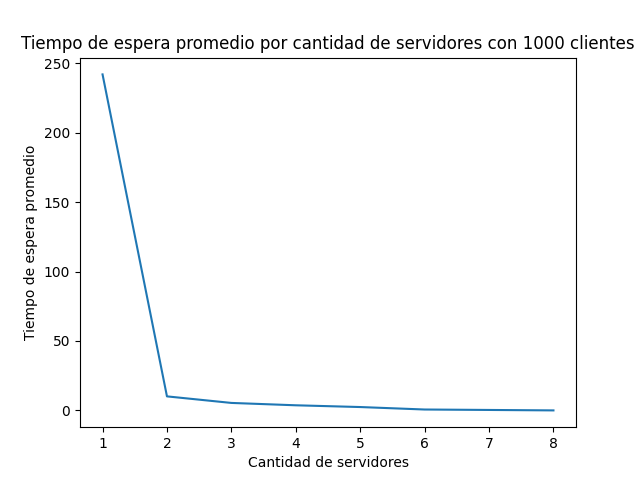
\includegraphics[scale=0.5]{../assets/Tiempo de espera promedio por cantidad de servidores con 1000 clientes.png}
\end{center}
\lstinputlisting[]{1000.txt}
\newpage
\item \textbf{Cantidad de clientes: 10000}
\begin{center}
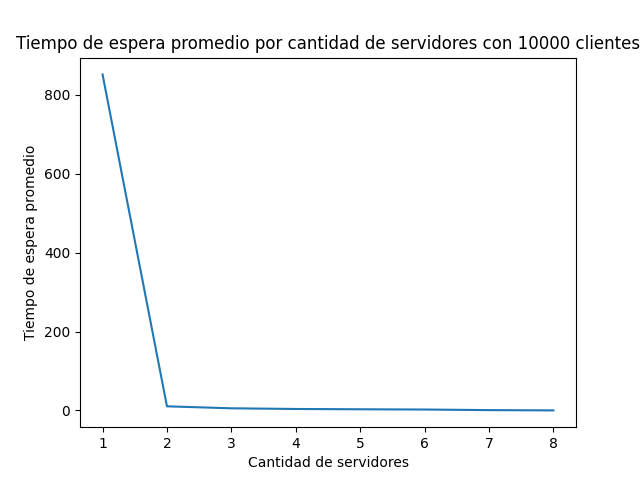
\includegraphics[scale=0.5]{../assets/Tiempo de espera promedio por cantidad de servidores con 10000 clientes.png}
\end{center}
\lstinputlisting[]{10000.txt}
\end{itemize}


\end{itemize}

\newpage
\section{Modelo matem\'atico}

\begin{enumerate}
\item \textbf{Descripción del modelo de simulación}\\
    La llegada de un cliente se simula tomando el momento de llegada del \'ultimo cliente, se genera un entero que distribuya M, se actualiza el estado de la simulaci\'on hasta el momento de llegada del \'ultimo cliente m\'as el tiempo que tard\'o el cliente actual en llegar y si no hay servidores activos se agrega el nuevo cliente a la cola, si en cambio hay alg\'un servidor activo se le asigna al cliente actual.\\
    La asignaci\'on de un servidor a un cliente consiste en eliminar el servidor de los servidores activos, y agregarlo junto con el momento en el cual terminar\'a de realizar el servicio al conjunto de los servidores ocupados. El momento en el cual terminar\'a de realizar el servicio es: momento actual m\'as n\'umero aleatorio generado seg\'un la distribuci\'on del servidor.\\
    La salida de los clientes se realiza cuando se actualiza el estado de la simulaci\'on tras actualizar el momento actual de la misma. Se comprueba si el momento de terminar el servicio ya pas\'o y se elimina el servidor del conjunto de servidores ocupados y se agrega al conjunto de servidores activos.\\

\item \textbf{Supuestos y restricciones}\\
Los eventos de llegada se simulan como una variable aleatoria completamente independiente para cada cliente que arriba.\\
Definición de los supuestos del modelo, como la independencia de los eventos de llegada y la asincronicidad de los servicios.\\

La simulación de eventos discretos se refiere a la técnica de modelar y analizar sistemas complejos mediante la simulación de eventos individuales que ocurren en el tiempo. En el contexto de un sistema con (n) servidores en paralelo y una cola para los clientes, esta técnica permite estudiar el flujo de trabajo, la eficiencia del sistema y el comportamiento bajo diferentes condiciones.\\
\item \textbf{Componentes del Modelo}\\
\begin{itemize}

\item    \textbf{Servidores}: (n) servidores operan en paralelo. Cada servidor puede atender a un cliente a la vez. Los servidores pueden tener diferentes tiempos de servicio.\\
\item    \textbf{Cola de Clientes}: Los clientes llegan al sistema y esperan en una cola para ser atendidos. La cola tiene una capacidad máxima, y si la cola está llena, los clientes adicionales se rechazan o deben esperar hasta que haya espacio disponible.\\

\end{itemize}
\item \textbf{Modelado Matemático}\\

El modelo matemático para este sistema se basa en la simulación de eventos discretos, donde cada evento (llegada de un cliente, servicio de un cliente, liberación de un servidor) se modela como un evento discreto en el tiempo.\\

    Eventos de Llegada: Los clientes llegan al sistema con una distribución de probabilidad exponencial, indicando el tiempo entre llegadas sucesivas.\\
    Eventos de Servicio: Cuando un servidor está libre, puede comenzar a atender a un cliente. El tiempo de servicio se modela de manera similar a los tiempos de llegada, utilizando una distribución exponencial.\\
    Eventos de Liberación: Cuando un servidor ha terminado de atender a un cliente, se libera para atender al siguiente cliente en la cola o para esperar a que llegue un nuevo cliente.\\

\item \textbf{Algoritmo de Simulación}\\

La simulación se realiza mediante un algoritmo que mantiene un registro de los eventos futuros y actualiza el estado del sistema (número de clientes en la cola, servidores ocupados, etc.) según ocurran estos eventos. Aquí hay un esquema básico del algoritmo:\\

    Inicialización: Se establece el estado inicial del sistema, incluyendo el tiempo actual(0) y el número de servidores libres(inicialmente todos).\\
    Llegada de un nuevo cliente: Se genera el momento de llegada del cliente y se actualiza el estado de la simulaci\'on, luego se simula la atenci\'on a ese cliente.
    Actualizaci\'on del estado de la simulaci\'on: Dado un tiempo se actualiza el estado de la simulaci\'on sacando a todos los clientes que terminaban derecibir su servico antes del momento actual  y a la vez se van procesando los clientes que estuviesen en la cola.
    Repetición: Se repite el proceso para el siguiente cliente hasta que se terminen de procesar todos.\\

\item \textbf{Ventajas y Aplicaciones}\\

Este modelo matemático es útil para analizar y optimizar sistemas de colas y servidores, como líneas de montaje, centros de llamadas, y sistemas de procesamiento de transacciones. Permite evaluar el rendimiento del sistema bajo diferentes condiciones y entender cómo los cambios en el sistema (por ejemplo, aumentar el número de servidores o modificar los tiempos de servicio) afectan la eficiencia y el tiempo de espera de los clientes.\\

La simulación de eventos discretos es una herramienta poderosa para el análisis de sistemas complejos, proporcionando una visión detallada del comportamiento del sistema en tiempo real y permitiendo experimentar con diferentes políticas y configuraciones sin el costo y riesgo asociado con la implementación en el mundo real\\



\end{enumerate}

\end{document}
